% Options for packages loaded elsewhere
\PassOptionsToPackage{unicode}{hyperref}
\PassOptionsToPackage{hyphens}{url}
%
\documentclass[
]{article}
\usepackage{lmodern}
\usepackage{amssymb,amsmath}
\usepackage{ifxetex,ifluatex}
\ifnum 0\ifxetex 1\fi\ifluatex 1\fi=0 % if pdftex
  \usepackage[T1]{fontenc}
  \usepackage[utf8]{inputenc}
  \usepackage{textcomp} % provide euro and other symbols
\else % if luatex or xetex
  \usepackage{unicode-math}
  \defaultfontfeatures{Scale=MatchLowercase}
  \defaultfontfeatures[\rmfamily]{Ligatures=TeX,Scale=1}
\fi
% Use upquote if available, for straight quotes in verbatim environments
\IfFileExists{upquote.sty}{\usepackage{upquote}}{}
\IfFileExists{microtype.sty}{% use microtype if available
  \usepackage[]{microtype}
  \UseMicrotypeSet[protrusion]{basicmath} % disable protrusion for tt fonts
}{}
\makeatletter
\@ifundefined{KOMAClassName}{% if non-KOMA class
  \IfFileExists{parskip.sty}{%
    \usepackage{parskip}
  }{% else
    \setlength{\parindent}{0pt}
    \setlength{\parskip}{6pt plus 2pt minus 1pt}}
}{% if KOMA class
  \KOMAoptions{parskip=half}}
\makeatother
\usepackage{xcolor}
\IfFileExists{xurl.sty}{\usepackage{xurl}}{} % add URL line breaks if available
\IfFileExists{bookmark.sty}{\usepackage{bookmark}}{\usepackage{hyperref}}
\hypersetup{
  pdftitle={GMSE ongoing analysis},
  pdfauthor={Matt Nuttall},
  hidelinks,
  pdfcreator={LaTeX via pandoc}}
\urlstyle{same} % disable monospaced font for URLs
\usepackage[margin=1in]{geometry}
\usepackage{color}
\usepackage{fancyvrb}
\newcommand{\VerbBar}{|}
\newcommand{\VERB}{\Verb[commandchars=\\\{\}]}
\DefineVerbatimEnvironment{Highlighting}{Verbatim}{commandchars=\\\{\}}
% Add ',fontsize=\small' for more characters per line
\usepackage{framed}
\definecolor{shadecolor}{RGB}{48,48,48}
\newenvironment{Shaded}{\begin{snugshade}}{\end{snugshade}}
\newcommand{\AlertTok}[1]{\textcolor[rgb]{1.00,0.81,0.69}{#1}}
\newcommand{\AnnotationTok}[1]{\textcolor[rgb]{0.50,0.62,0.50}{\textbf{#1}}}
\newcommand{\AttributeTok}[1]{\textcolor[rgb]{0.80,0.80,0.80}{#1}}
\newcommand{\BaseNTok}[1]{\textcolor[rgb]{0.86,0.64,0.64}{#1}}
\newcommand{\BuiltInTok}[1]{\textcolor[rgb]{0.80,0.80,0.80}{#1}}
\newcommand{\CharTok}[1]{\textcolor[rgb]{0.86,0.64,0.64}{#1}}
\newcommand{\CommentTok}[1]{\textcolor[rgb]{0.50,0.62,0.50}{#1}}
\newcommand{\CommentVarTok}[1]{\textcolor[rgb]{0.50,0.62,0.50}{\textbf{#1}}}
\newcommand{\ConstantTok}[1]{\textcolor[rgb]{0.86,0.64,0.64}{\textbf{#1}}}
\newcommand{\ControlFlowTok}[1]{\textcolor[rgb]{0.94,0.87,0.69}{#1}}
\newcommand{\DataTypeTok}[1]{\textcolor[rgb]{0.87,0.87,0.75}{#1}}
\newcommand{\DecValTok}[1]{\textcolor[rgb]{0.86,0.86,0.80}{#1}}
\newcommand{\DocumentationTok}[1]{\textcolor[rgb]{0.50,0.62,0.50}{#1}}
\newcommand{\ErrorTok}[1]{\textcolor[rgb]{0.76,0.75,0.62}{#1}}
\newcommand{\ExtensionTok}[1]{\textcolor[rgb]{0.80,0.80,0.80}{#1}}
\newcommand{\FloatTok}[1]{\textcolor[rgb]{0.75,0.75,0.82}{#1}}
\newcommand{\FunctionTok}[1]{\textcolor[rgb]{0.94,0.94,0.56}{#1}}
\newcommand{\ImportTok}[1]{\textcolor[rgb]{0.80,0.80,0.80}{#1}}
\newcommand{\InformationTok}[1]{\textcolor[rgb]{0.50,0.62,0.50}{\textbf{#1}}}
\newcommand{\KeywordTok}[1]{\textcolor[rgb]{0.94,0.87,0.69}{#1}}
\newcommand{\NormalTok}[1]{\textcolor[rgb]{0.80,0.80,0.80}{#1}}
\newcommand{\OperatorTok}[1]{\textcolor[rgb]{0.94,0.94,0.82}{#1}}
\newcommand{\OtherTok}[1]{\textcolor[rgb]{0.94,0.94,0.56}{#1}}
\newcommand{\PreprocessorTok}[1]{\textcolor[rgb]{1.00,0.81,0.69}{\textbf{#1}}}
\newcommand{\RegionMarkerTok}[1]{\textcolor[rgb]{0.80,0.80,0.80}{#1}}
\newcommand{\SpecialCharTok}[1]{\textcolor[rgb]{0.86,0.64,0.64}{#1}}
\newcommand{\SpecialStringTok}[1]{\textcolor[rgb]{0.80,0.58,0.58}{#1}}
\newcommand{\StringTok}[1]{\textcolor[rgb]{0.80,0.58,0.58}{#1}}
\newcommand{\VariableTok}[1]{\textcolor[rgb]{0.80,0.80,0.80}{#1}}
\newcommand{\VerbatimStringTok}[1]{\textcolor[rgb]{0.80,0.58,0.58}{#1}}
\newcommand{\WarningTok}[1]{\textcolor[rgb]{0.50,0.62,0.50}{\textbf{#1}}}
\usepackage{longtable,booktabs}
% Correct order of tables after \paragraph or \subparagraph
\usepackage{etoolbox}
\makeatletter
\patchcmd\longtable{\par}{\if@noskipsec\mbox{}\fi\par}{}{}
\makeatother
% Allow footnotes in longtable head/foot
\IfFileExists{footnotehyper.sty}{\usepackage{footnotehyper}}{\usepackage{footnote}}
\makesavenoteenv{longtable}
\usepackage{graphicx,grffile}
\makeatletter
\def\maxwidth{\ifdim\Gin@nat@width>\linewidth\linewidth\else\Gin@nat@width\fi}
\def\maxheight{\ifdim\Gin@nat@height>\textheight\textheight\else\Gin@nat@height\fi}
\makeatother
% Scale images if necessary, so that they will not overflow the page
% margins by default, and it is still possible to overwrite the defaults
% using explicit options in \includegraphics[width, height, ...]{}
\setkeys{Gin}{width=\maxwidth,height=\maxheight,keepaspectratio}
% Set default figure placement to htbp
\makeatletter
\def\fps@figure{htbp}
\makeatother
\setlength{\emergencystretch}{3em} % prevent overfull lines
\providecommand{\tightlist}{%
  \setlength{\itemsep}{0pt}\setlength{\parskip}{0pt}}
\setcounter{secnumdepth}{-\maxdimen} % remove section numbering

\title{GMSE ongoing analysis}
\author{Matt Nuttall}
\date{30/10/20}

\begin{document}
\maketitle

{
\setcounter{tocdepth}{2}
\tableofcontents
}
This is a summary of my ongoing GMSE analysis which will investigate the
social-ecological dynamics surrounding land tenure in a hypothetical
conservation landscape that is loosely based on a Cambodian protected
area.

As discussed, I have started simple and will build complexity as I go.

I have started with a landscape as follows:

\begin{itemize}
\tightlist
\item
  The landscape dimensions are 50 x 50. I am assuming that a cell
  represents 1 ha, and therefore this landscape is currently 2500 ha /
  25km\^{}2. I will increase the size of the landscape later, but I am
  keeping it small at the moment to reduce run time.
\item
  There are 50 individual users. This can represent a community of 50
  families. Currently users act independently.
\item
  Land ownership is currently FALSE
\item
  Users can move around the landscape
\item
  I have found papers that report tree density in tropical forest
  landscapes, and they vary widely. One paper (Sagar \& Singh 2006
  \url{https://www.jstor.org/stable/44521915}) report a range between 35
  and 419 stems per ha. To keep run time low I have started with 50
  trees/ha. This is low but not implausible. This can be increased
  later.
\item
  The manager has imperfect detection.
\end{itemize}

I have started with managers wanting to preserve all trees, but having
very little power to set policy. In later simulations I have increased
the manager budget a bit, and then started increasing manager budgets to
see where the threshold for reducing clearance is.

\hypertarget{simulation-0-ten_rep_0}{%
\subsection{Simulation 0 (ten\_rep\_0)}\label{simulation-0-ten_rep_0}}

Here I have set res\_consume = 0. I wanted to start with the presence of
trees on a cell not impacting yield at all, i.e.~to remove any incentive
for the users to clear forest. Although Brad has since confirmed that
when land\_ownership = FALSE then the users are essentially hunters and
will try to cull as much as possible regardless of the effect of trees
on yield.

Model set up:

\begin{Shaded}
\begin{Highlighting}[]
\NormalTok{ten_rep_}\DecValTok{0}\NormalTok{ <-}\StringTok{ }\KeywordTok{gmse}\NormalTok{(}
  \DataTypeTok{time_max =} \DecValTok{40}\NormalTok{,}
  \DataTypeTok{land_dim_1 =} \DecValTok{50}\NormalTok{,}
  \DataTypeTok{land_dim_2 =} \DecValTok{50}\NormalTok{, }\CommentTok{# landscape is 2500ha or 25km2}
  \DataTypeTok{res_movement =} \DecValTok{0}\NormalTok{, }\CommentTok{# trees don't move }
  \DataTypeTok{remove_pr =} \DecValTok{0}\NormalTok{, }\CommentTok{# Assume no death }
  \DataTypeTok{lambda =} \DecValTok{0}\NormalTok{, }\CommentTok{# assume no growth}
  \DataTypeTok{agent_view =} \DecValTok{10}\NormalTok{, }\CommentTok{# distance (cells) agent can see (currently only manager during obs process)}
  \DataTypeTok{agent_move =} \DecValTok{50}\NormalTok{, }\CommentTok{# distance (cells) agents can travel (mostly affects managers during obs process)}
  \DataTypeTok{res_birth_K =} \DecValTok{1}\NormalTok{, }\CommentTok{# must be positive value, but I want it small i.e. no real recruitment}
  \DataTypeTok{res_death_K =} \DecValTok{500000}\NormalTok{, }\CommentTok{# carrying capacity set to way above starting number of resources}
  \DataTypeTok{res_move_type =} \DecValTok{0}\NormalTok{, }\CommentTok{# 0=no move, }
  \DataTypeTok{res_death_type =} \DecValTok{1}\NormalTok{, }\CommentTok{# 1=density-independent }
  \DataTypeTok{observe_type =} \DecValTok{0}\NormalTok{, }\CommentTok{# 0=density-based sampling }
  \DataTypeTok{times_observe =} \DecValTok{1}\NormalTok{, }\CommentTok{# observes once}
  \DataTypeTok{obs_move_type =} \DecValTok{1}\NormalTok{, }\CommentTok{# uniform in any direction}
  \DataTypeTok{res_min_age =} \DecValTok{0}\NormalTok{, }\CommentTok{# age of resources before agents record/act on them}
  \DataTypeTok{res_move_obs =} \OtherTok{FALSE}\NormalTok{, }\CommentTok{# trees don't move}
  \DataTypeTok{plotting =} \OtherTok{FALSE}\NormalTok{, }
  \DataTypeTok{res_consume =} \DecValTok{0}\NormalTok{, }\CommentTok{# trees have no impact on yield}
  
  \CommentTok{# all genetic algorithm parameters left to default}
  
  \DataTypeTok{move_agents =} \OtherTok{TRUE}\NormalTok{, }\CommentTok{# should agents move at the end of each time step?}
  \DataTypeTok{max_ages =} \DecValTok{1000}\NormalTok{, }\CommentTok{# maximum ages of resources - set very high to reduce natural death}
  \DataTypeTok{user_budget =} \DecValTok{1000}\NormalTok{, }\CommentTok{# total budget of each stakeholder for performing actions}
  \DataTypeTok{manager_budget =} \DecValTok{500}\NormalTok{, }\CommentTok{# Manager has little power (50% of user)}
  \DataTypeTok{manage_target =} \DecValTok{125000}\NormalTok{, }\CommentTok{# target resource abundance (same as starting value)}
  \DataTypeTok{RESOURCE_ini =} \DecValTok{125000}\NormalTok{, }\CommentTok{# initial abundance of resources - 50 trees per cell}
  \DataTypeTok{culling =} \OtherTok{TRUE}\NormalTok{, }\CommentTok{# culling is only option}
  \DataTypeTok{tend_crops =} \OtherTok{FALSE}\NormalTok{, }\CommentTok{# is tending crops on landscape allowed. if TRUE, user can increase yield each time step}
  \DataTypeTok{stakeholders =} \DecValTok{30}\NormalTok{, }\CommentTok{# a village with 50 families}
  \DataTypeTok{land_ownership =} \OtherTok{FALSE}\NormalTok{, }\CommentTok{# no land ownership}
  \DataTypeTok{group_think =} \OtherTok{FALSE} \CommentTok{# users act independently}
\NormalTok{)}
\end{Highlighting}
\end{Shaded}

\begin{verbatim}
## [1] "Initialising simulations ... "
## [1] "Generation  1 of  40"
## [1] "Generation  2 of  40"
## [1] "Generation  3 of  40"
## [1] "Generation  4 of  40"
## [1] "Generation  5 of  40"
## [1] "Generation  6 of  40"
## [1] "Generation  7 of  40"
## [1] "Generation  8 of  40"
## [1] "Generation  9 of  40"
## [1] "Generation  10 of  40"
## [1] "Generation  11 of  40"
## [1] "Generation  12 of  40"
## [1] "Generation  13 of  40"
## [1] "Generation  14 of  40"
## [1] "Generation  15 of  40"
## [1] "Generation  16 of  40"
## [1] "Generation  17 of  40"
## [1] "Generation  18 of  40"
## [1] "Generation  19 of  40"
## [1] "Generation  20 of  40"
## [1] "Generation  21 of  40"
## [1] "Generation  22 of  40"
## [1] "Generation  23 of  40"
## [1] "Generation  24 of  40"
## [1] "Generation  25 of  40"
## [1] "Generation  26 of  40"
## [1] "Generation  27 of  40"
## [1] "Generation  28 of  40"
## [1] "Generation  29 of  40"
## [1] "Generation  30 of  40"
## [1] "Generation  31 of  40"
## [1] "Generation  32 of  40"
## [1] "Generation  33 of  40"
## [1] "Generation  34 of  40"
## [1] "Generation  35 of  40"
## [1] "Generation  36 of  40"
## [1] "Generation  37 of  40"
## [1] "Generation  38 of  40"
## [1] "Generation  39 of  40"
## [1] "Generation  40 of  40"
\end{verbatim}

\includegraphics{gmse_tenure_ongoing_files/figure-latex/ten_rep_0_plot-1.pdf}

This is not what I was initially expecting. I had assumed that if there
was no impact on yield, then users would have no incentive to cull
trees. But thanks to Brad's explanation, this is now clear.

\hypertarget{simulations-1-and-2-ten_rep_1-ten_rep_2}{%
\subsection{Simulations 1 and 2 (ten\_rep\_1,
ten\_rep\_2)}\label{simulations-1-and-2-ten_rep_1-ten_rep_2}}

In these simulations I have changed res\_consume to 0.02. So for now I
am saying each tree reduces cell yield by 2\%. This means that if there
are 50 trees on a cell, then yield is reduced to 0.36\% of the total
(vaguely plausible for an open forest e.g.~deciduous diptercarp
landscape). Cutting down 10 trees (20\% of the trees) increases yield to
0.44, cutting down 20 trees (40\%) increases yield to 0.54\% etc. This
is assuming I have correctly understood the exponential function Brad
sent: yield = (1 - \%yield reduction per tree)\^{}remaining trees

First I will run a single call of gmse() with 40 time steps. Then I will
use gmse\_replicate() to run the simulation 10 times to see the
variation in outcomes.

\hypertarget{single-call}{%
\subsubsection{Single call}\label{single-call}}

Model set up:

\begin{Shaded}
\begin{Highlighting}[]
\NormalTok{ten_rep_}\DecValTok{1}\NormalTok{ <-}\StringTok{ }\KeywordTok{gmse}\NormalTok{(}
  \DataTypeTok{time_max =} \DecValTok{40}\NormalTok{,}
  \DataTypeTok{land_dim_1 =} \DecValTok{50}\NormalTok{,}
  \DataTypeTok{land_dim_2 =} \DecValTok{50}\NormalTok{, }\CommentTok{# landscape is 2500ha or 25km2}
  \DataTypeTok{res_movement =} \DecValTok{0}\NormalTok{, }\CommentTok{# trees don't move }
  \DataTypeTok{remove_pr =} \DecValTok{0}\NormalTok{, }\CommentTok{# Assume no death }
  \DataTypeTok{lambda =} \DecValTok{0}\NormalTok{, }\CommentTok{# assume no growth}
  \DataTypeTok{agent_view =} \DecValTok{10}\NormalTok{, }\CommentTok{# distance (cells) agent can see (currently only manager during obs process)}
  \DataTypeTok{agent_move =} \DecValTok{50}\NormalTok{, }\CommentTok{# distance (cells) agents can travel (mostly affects managers during obs process)}
  \DataTypeTok{res_birth_K =} \DecValTok{1}\NormalTok{, }\CommentTok{# must be positive value, but I want it small i.e. no real recruitment}
  \DataTypeTok{res_death_K =} \DecValTok{500000}\NormalTok{, }\CommentTok{# carrying capacity set to way above starting number of resources}
  \DataTypeTok{res_move_type =} \DecValTok{0}\NormalTok{, }\CommentTok{# 0=no move, }
  \DataTypeTok{res_death_type =} \DecValTok{1}\NormalTok{, }\CommentTok{# 1=density-independent }
  \DataTypeTok{observe_type =} \DecValTok{0}\NormalTok{, }\CommentTok{# 0=density-based sampling }
  \DataTypeTok{times_observe =} \DecValTok{1}\NormalTok{, }\CommentTok{# observes once}
  \DataTypeTok{obs_move_type =} \DecValTok{1}\NormalTok{, }\CommentTok{# uniform in any direction}
  \DataTypeTok{res_min_age =} \DecValTok{0}\NormalTok{, }\CommentTok{# age of resources before agents record/act on them}
  \DataTypeTok{res_move_obs =} \OtherTok{FALSE}\NormalTok{, }\CommentTok{# trees don't move}
  \DataTypeTok{plotting =} \OtherTok{FALSE}\NormalTok{, }
  \DataTypeTok{res_consume =} \FloatTok{0.02}\NormalTok{,}
  
  \CommentTok{# all genetic algorithm parameters left to default}
  
  \DataTypeTok{move_agents =} \OtherTok{TRUE}\NormalTok{, }\CommentTok{# should agents move at the end of each time step?}
  \DataTypeTok{max_ages =} \DecValTok{1000}\NormalTok{, }\CommentTok{# maximum ages of resources - set very high to reduce natural death}
  \DataTypeTok{minimum_cost =} \DecValTok{10}\NormalTok{, }\CommentTok{# minimum cost of any action in user & manager models - improves precision of manager policy(?)}
  \DataTypeTok{user_budget =} \DecValTok{1000}\NormalTok{, }\CommentTok{# total budget of each stakeholder for performing actions}
  \DataTypeTok{manager_budget =} \DecValTok{100}\NormalTok{, }\CommentTok{# Manager has very little power (10% of user)}
  \DataTypeTok{manage_target =} \DecValTok{125000}\NormalTok{, }\CommentTok{# target resource abundance (same as starting value)}
  \DataTypeTok{RESOURCE_ini =} \DecValTok{125000}\NormalTok{, }\CommentTok{# initial abundance of resources - 50 trees per cell}
  \DataTypeTok{culling =} \OtherTok{TRUE}\NormalTok{, }\CommentTok{# culling is only option}
  \DataTypeTok{tend_crops =} \OtherTok{FALSE}\NormalTok{, }\CommentTok{# is tending crops on landscape allowed. if TRUE, user can increase yield each time step}
  \DataTypeTok{stakeholders =} \DecValTok{50}\NormalTok{, }\CommentTok{# a village with 50 families}
  \DataTypeTok{land_ownership =} \OtherTok{FALSE}\NormalTok{, }\CommentTok{# no land ownership}
  \DataTypeTok{manage_freq =} \DecValTok{1}\NormalTok{, }\CommentTok{# frequency of manager setting policy }
  \DataTypeTok{group_think =} \OtherTok{FALSE} \CommentTok{# users act independently}
\NormalTok{)}
\end{Highlighting}
\end{Shaded}

\begin{verbatim}
## [1] "Initialising simulations ... "
## [1] "Generation  1 of  40"
## [1] "Generation  2 of  40"
## [1] "Generation  3 of  40"
## [1] "Generation  4 of  40"
## [1] "Generation  5 of  40"
## [1] "Generation  6 of  40"
## [1] "Generation  7 of  40"
## [1] "Generation  8 of  40"
## [1] "Generation  9 of  40"
## [1] "Generation  10 of  40"
## [1] "Generation  11 of  40"
## [1] "Generation  12 of  40"
## [1] "Generation  13 of  40"
## [1] "Generation  14 of  40"
## [1] "Generation  15 of  40"
## [1] "Generation  16 of  40"
## [1] "Generation  17 of  40"
## [1] "Generation  18 of  40"
## [1] "Generation  19 of  40"
## [1] "Generation  20 of  40"
## [1] "Generation  21 of  40"
## [1] "Generation  22 of  40"
## [1] "Generation  23 of  40"
## [1] "Generation  24 of  40"
## [1] "Generation  25 of  40"
## [1] "Generation  26 of  40"
## [1] "Generation  27 of  40"
## [1] "Generation  28 of  40"
## [1] "Generation  29 of  40"
## [1] "Generation  30 of  40"
## [1] "Generation  31 of  40"
## [1] "Generation  32 of  40"
## [1] "Generation  33 of  40"
## [1] "Generation  34 of  40"
## [1] "Generation  35 of  40"
## [1] "Generation  36 of  40"
## [1] "Generation  37 of  40"
## [1] "Generation  38 of  40"
## [1] "Generation  39 of  40"
## [1] "Generation  40 of  40"
\end{verbatim}

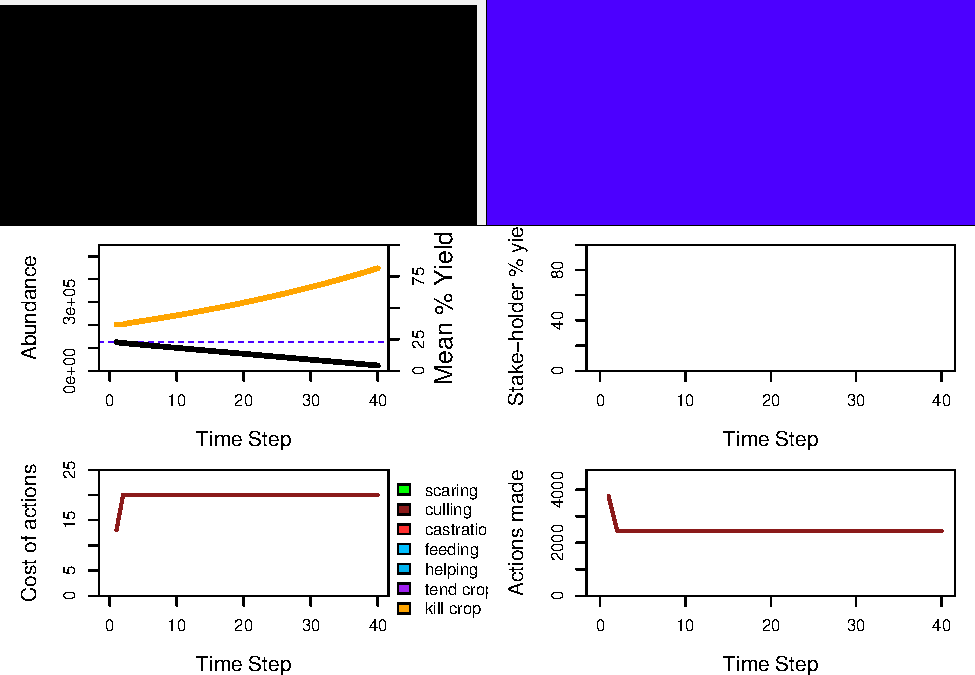
\includegraphics{gmse_tenure_ongoing_files/figure-latex/ten_rep_1_plot-1.pdf}

Here we see what I was expecting. The manager uses what little power
they have to prevent culling, but is not very effective. Users want to
reduce the trees in the cells as they are reducing yield. As trees are
culled, the resource population declines and the users yield increases.

The number of trees each user is harvesting per time step after the
costs have been increased is 50. In reality probably a bit low as a
family can clear more than that in a year (if we are assuming a time
step is a year). But fine for now.

\hypertarget{replicate-calls}{%
\subsubsection{Replicate calls}\label{replicate-calls}}

Here I repeat the above call 10 times and extract summary data. The
model set up is the same as above, just using gmse\_replicates()

\begin{Shaded}
\begin{Highlighting}[]
\NormalTok{knitr}\OperatorTok{::}\KeywordTok{kable}\NormalTok{(ten_rep_}\DecValTok{2}\NormalTok{_summary)}
\end{Highlighting}
\end{Shaded}

\begin{longtable}[]{@{}rrrrrrrrr@{}}
\toprule
X & time\_step & resources & estimate & cost\_culling & cost\_unused &
act\_culling & act\_unused & harvested\tabularnewline
\midrule
\endhead
1 & 40 & 22197 & 22103.17 & 20 & 0 & 2500 & 0 & 2500\tabularnewline
2 & 40 & 22898 & 22692.74 & 20 & 0 & 2500 & 0 & 2500\tabularnewline
3 & 40 & 23177 & 22715.42 & 20 & 0 & 2500 & 0 & 2500\tabularnewline
4 & 40 & 23959 & 24467.12 & 20 & 0 & 2500 & 0 & 2500\tabularnewline
5 & 40 & 23211 & 23106.58 & 20 & 0 & 2500 & 0 & 2500\tabularnewline
6 & 40 & 23730 & 23401.36 & 20 & 0 & 2500 & 0 & 2500\tabularnewline
7 & 40 & 23550 & 23690.48 & 20 & 0 & 2500 & 0 & 2500\tabularnewline
8 & 40 & 24333 & 24195.01 & 20 & 0 & 2500 & 0 & 2500\tabularnewline
9 & 40 & 23483 & 23276.64 & 20 & 0 & 2500 & 0 & 2500\tabularnewline
10 & 40 & 23693 & 23458.05 & 20 & 0 & 2500 & 0 & 2500\tabularnewline
\bottomrule
\end{longtable}

The amount of forest remaining at the end of each simulation is very
similar, and the costs and actions do not appear to vary.

\hypertarget{simulations-3-4-ten_rep_3-ten_rep_4}{%
\subsection{Simulations 3 \& 4 (ten\_rep\_3,
ten\_rep\_4)}\label{simulations-3-4-ten_rep_3-ten_rep_4}}

Here the model set up is identical to the above, but I have increased
the manager budget from 100 (10\% of user budget) to 500 (50\% of user
budget)

\hypertarget{single-call-1}{%
\subsubsection{Single call}\label{single-call-1}}

First I ran a single gmse() call

\begin{verbatim}
## [1] "Initialising simulations ... "
## [1] "Generation  1 of  40"
## [1] "Generation  2 of  40"
## [1] "Generation  3 of  40"
## [1] "Generation  4 of  40"
## [1] "Generation  5 of  40"
## [1] "Generation  6 of  40"
## [1] "Generation  7 of  40"
## [1] "Generation  8 of  40"
## [1] "Generation  9 of  40"
## [1] "Generation  10 of  40"
## [1] "Generation  11 of  40"
## [1] "Generation  12 of  40"
## [1] "Generation  13 of  40"
## [1] "Generation  14 of  40"
## [1] "Generation  15 of  40"
## [1] "Generation  16 of  40"
## [1] "Generation  17 of  40"
## [1] "Generation  18 of  40"
## [1] "Generation  19 of  40"
## [1] "Generation  20 of  40"
## [1] "Generation  21 of  40"
## [1] "Generation  22 of  40"
## [1] "Generation  23 of  40"
## [1] "Generation  24 of  40"
## [1] "Generation  25 of  40"
## [1] "Generation  26 of  40"
## [1] "Generation  27 of  40"
## [1] "Generation  28 of  40"
## [1] "Generation  29 of  40"
## [1] "Generation  30 of  40"
## [1] "Generation  31 of  40"
## [1] "Generation  32 of  40"
## [1] "Generation  33 of  40"
## [1] "Generation  34 of  40"
## [1] "Generation  35 of  40"
## [1] "Generation  36 of  40"
## [1] "Generation  37 of  40"
## [1] "Generation  38 of  40"
## [1] "Generation  39 of  40"
## [1] "Generation  40 of  40"
\end{verbatim}

\includegraphics{gmse_tenure_ongoing_files/figure-latex/ten_rep_3_plot-1.pdf}

Here we see the loss of trees is much less than before, as the manager
has more power to reduce culling by setting higher costs. Users are
still able to clear forest though, with 800 trees being lost each time
step once the manager has applied their policy.

\hypertarget{replicate-calls-1}{%
\subsubsection{Replicate calls}\label{replicate-calls-1}}

\includegraphics{gmse_tenure_ongoing_files/figure-latex/ten_rep_4_plot_resources-1.pdf}

There is not much variation in the decline in resources. I guess this is
because the model currently has little flexibility - the manager will
always set the highest cost possible as they are trying to maintain all
resources, and the users will always try to cull. Furthermore the
resources are not reproducing or naturally dying (much), and so there is
not much stochasticity in the resource population. Therefore after the
inital setting of policy in time step 1, there will be little change
between the simulations.

We do however, see some variation in the initial number of culling
actions (see below plot)

\includegraphics{gmse_tenure_ongoing_files/figure-latex/ten_rep_4_plot_actions-1.pdf}

I was not clear what was behind this variation. I thought perhaps it was
driven by the fact that, by chance, some users will find themselves on a
cell with more resources than othes. Brad has since clarified that this
is proabbly due to the genetic algorithm not finding the optimal
harvesting solution right away (or the users taking a time step to
``learn'').

\hypertarget{simulation-5-ten_rep_5}{%
\subsection{Simulation 5 (ten\_rep\_5)}\label{simulation-5-ten_rep_5}}

Here I have used gmse\_apply() to dynamically change the managers
budget. I have increased the manager budget incrementally over the 40
time steps, in quantities that mean the manager budget exceeds the user
budget at some point during the time period.

I would like to see what effects increasing manager budgets have on the
actions of the users, and on the resources. I would also like to see how
large the manager's budget needs to be to completely stop all culling.

Model set up:

\begin{Shaded}
\begin{Highlighting}[]
\CommentTok{# manager budget}
\NormalTok{mb <-}\StringTok{ }\DecValTok{500}

\CommentTok{# sim_old}
\NormalTok{ten_rep_}\DecValTok{5}\NormalTok{_simold <-}\StringTok{ }\KeywordTok{gmse_apply}\NormalTok{(}
  \DataTypeTok{res_mod =}\NormalTok{ resource,}
  \DataTypeTok{obs_mod =}\NormalTok{ observation,}
  \DataTypeTok{man_mod =}\NormalTok{ manager,}
  \DataTypeTok{use_mod =}\NormalTok{ user,}
  \DataTypeTok{get_res =} \StringTok{"FUll"}\NormalTok{,}
  \DataTypeTok{land_dim_1 =} \DecValTok{50}\NormalTok{,}
  \DataTypeTok{land_dim_2 =} \DecValTok{50}\NormalTok{, }\CommentTok{# landscape is 2500ha or 25km2}
  \DataTypeTok{res_movement =} \DecValTok{0}\NormalTok{, }\CommentTok{# trees don't move }
  \DataTypeTok{remove_pr =} \DecValTok{0}\NormalTok{, }\CommentTok{# Assume no death }
  \DataTypeTok{lambda =} \DecValTok{0}\NormalTok{, }\CommentTok{# assume no growth}
  \DataTypeTok{agent_view =} \DecValTok{10}\NormalTok{, }\CommentTok{# distance (cells) agent can see (currently only manager during obs process)}
  \DataTypeTok{agent_move =} \DecValTok{50}\NormalTok{, }\CommentTok{# distance (cells) agents can travel (mostly affects managers during obs process)}
  \DataTypeTok{res_birth_K =} \DecValTok{1}\NormalTok{, }\CommentTok{# must be positive value, but I want it small i.e. no real recruitment}
  \DataTypeTok{res_death_K =} \DecValTok{500000}\NormalTok{, }\CommentTok{# carrying capacity set to way above starting number of resources}
  \DataTypeTok{res_move_type =} \DecValTok{0}\NormalTok{, }\CommentTok{# 0=no move, }
  \DataTypeTok{res_death_type =} \DecValTok{1}\NormalTok{, }\CommentTok{# 1=density-independent }
  \DataTypeTok{observe_type =} \DecValTok{0}\NormalTok{, }\CommentTok{# 0=density-based sampling }
  \DataTypeTok{times_observe =} \DecValTok{1}\NormalTok{, }\CommentTok{# observes once}
  \DataTypeTok{obs_move_type =} \DecValTok{1}\NormalTok{, }\CommentTok{# uniform in any direction}
  \DataTypeTok{res_min_age =} \DecValTok{0}\NormalTok{, }\CommentTok{# age of resources before agents record/act on them}
  \DataTypeTok{res_move_obs =} \OtherTok{FALSE}\NormalTok{, }\CommentTok{# trees don't move}
  \DataTypeTok{plotting =} \OtherTok{FALSE}\NormalTok{, }
  \DataTypeTok{res_consume =} \FloatTok{0.02}\NormalTok{, }
  
  \CommentTok{# all genetic algorithm parameters left to default}
  
  \DataTypeTok{move_agents =} \OtherTok{TRUE}\NormalTok{, }\CommentTok{# should agents move at the end of each time step?}
  \DataTypeTok{max_ages =} \DecValTok{1000}\NormalTok{, }\CommentTok{# maximum ages of resources - set very high to reduce natural death}
  \DataTypeTok{user_budget =} \DecValTok{1000}\NormalTok{, }\CommentTok{# total budget of each stakeholder for performing actions}
  \DataTypeTok{manager_budget =}\NormalTok{ mb, }\CommentTok{# Manager has little power (50% of user)}
  \DataTypeTok{manage_target =} \DecValTok{125000}\NormalTok{, }\CommentTok{# target resource abundance (same as starting value)}
  \DataTypeTok{RESOURCE_ini =} \DecValTok{125000}\NormalTok{, }\CommentTok{# initial abundance of resources - 50 trees per cell}
  \DataTypeTok{culling =} \OtherTok{TRUE}\NormalTok{, }\CommentTok{# culling is only option}
  \DataTypeTok{tend_crops =} \OtherTok{FALSE}\NormalTok{, }\CommentTok{# is tending crops on landscape allowed. if TRUE, user can increase yield each time step}
  \DataTypeTok{stakeholders =} \DecValTok{50}\NormalTok{, }\CommentTok{# a village with 50 families}
\NormalTok{)}

\CommentTok{# matrix for results}
\NormalTok{ten_rep_}\DecValTok{5}\NormalTok{ <-}\StringTok{ }\KeywordTok{matrix}\NormalTok{(}\DataTypeTok{data=}\OtherTok{NA}\NormalTok{, }\DataTypeTok{nrow=}\DecValTok{40}\NormalTok{, }\DataTypeTok{ncol=}\DecValTok{6}\NormalTok{)}

\CommentTok{# loop the simulation. Took 11 mins}
\ControlFlowTok{for}\NormalTok{(time_step }\ControlFlowTok{in} \DecValTok{1}\OperatorTok{:}\DecValTok{40}\NormalTok{)\{}
  
\NormalTok{  sim_new <-}\StringTok{ }\KeywordTok{gmse_apply}\NormalTok{(}\DataTypeTok{get_res =} \StringTok{"Full"}\NormalTok{, }\DataTypeTok{old_list =}\NormalTok{ ten_rep_}\DecValTok{5}\NormalTok{_simold, }\DataTypeTok{manager_budget=}\NormalTok{mb)}
  
\NormalTok{  ten_rep_}\DecValTok{5}\NormalTok{[time_step, }\DecValTok{1}\NormalTok{] <-}\StringTok{ }\NormalTok{time_step}
\NormalTok{  ten_rep_}\DecValTok{5}\NormalTok{[time_step, }\DecValTok{2}\NormalTok{] <-}\StringTok{ }\NormalTok{sim_new}\OperatorTok{$}\NormalTok{basic_output}\OperatorTok{$}\NormalTok{resource_results[}\DecValTok{1}\NormalTok{]}
\NormalTok{  ten_rep_}\DecValTok{5}\NormalTok{[time_step, }\DecValTok{3}\NormalTok{] <-}\StringTok{ }\NormalTok{sim_new}\OperatorTok{$}\NormalTok{basic_output}\OperatorTok{$}\NormalTok{observation_results[}\DecValTok{1}\NormalTok{]}
\NormalTok{  ten_rep_}\DecValTok{5}\NormalTok{[time_step, }\DecValTok{4}\NormalTok{] <-}\StringTok{ }\NormalTok{sim_new}\OperatorTok{$}\NormalTok{basic_output}\OperatorTok{$}\NormalTok{manager_results[}\DecValTok{3}\NormalTok{]}
\NormalTok{  ten_rep_}\DecValTok{5}\NormalTok{[time_step, }\DecValTok{5}\NormalTok{] <-}\StringTok{ }\KeywordTok{sum}\NormalTok{(sim_new}\OperatorTok{$}\NormalTok{basic_output}\OperatorTok{$}\NormalTok{user_results[,}\DecValTok{3}\NormalTok{])}
\NormalTok{  ten_rep_}\DecValTok{5}\NormalTok{[time_step, }\DecValTok{6}\NormalTok{] <-}\StringTok{ }\NormalTok{mb}
  
\NormalTok{  ten_rep_}\DecValTok{5}\NormalTok{_simold <-}\StringTok{ }\NormalTok{sim_new}
\NormalTok{  mb <-}\StringTok{ }\NormalTok{mb }\OperatorTok{+}\StringTok{ }\DecValTok{20}
  
\NormalTok{\}}

\KeywordTok{colnames}\NormalTok{(ten_rep_}\DecValTok{5}\NormalTok{) <-}\StringTok{ }\KeywordTok{c}\NormalTok{(}\StringTok{"Time"}\NormalTok{, }\StringTok{"Pop_size"}\NormalTok{, }\StringTok{"Pop_est"}\NormalTok{, }\StringTok{"Cull_cost"}\NormalTok{, }\StringTok{"Cull_count"}\NormalTok{,}
                         \StringTok{"Manager_budget"}\NormalTok{)}
\end{Highlighting}
\end{Shaded}

Below are some exploratory plots.

\includegraphics{gmse_tenure_ongoing_files/figure-latex/ten_rep_5_summary-1.pdf}

The top left plot shows that there is a linear relationship between the
manager's budget and the cost of culling. In other words, because the
manager is trying to stop ALL culling, as soon as they have more budget
they will use it to increase the cost of culling.

The plot on the top right I was not quite expecting. There appear to be
budget/cost thresholds for increases in culling. This can be seen in the
``steps''. For a given manager budget/cull cost, there will be a certain
number of culling actions. The number of culling actions will stay the
same for a number of time steps, even when the manager budget (and
therefore the cost) increases. Then there will be a drop to another
level of culling actions. Interestingly, when manager budgets/costs are
relatively low, the count of culling actions decrease more quickly in
response to increases in cost. Whereas when costs are relatively high,
the number of culling actions stay at the same level for longer, despite
increases in cost. In other words, the manager's budget appears to have
a larger relative impact when it is lower. I am not sure why this is.

The bottom plot shows how the number of trees lost per time step
decreases as manager budgets increase. In other words, as the manager
gains power to enact policy, the fewer trees are lost. I guess the
stochasticity that can be seen is a result of the changes in the natural
die off of trees (otherwise I would expect to see steps, as in the top
right plot). The large decrease between time step 1 and 2 will be
presumably because the users will cull as much as possible in the
beginning before the manager increases the cost in the next time step.

I have clearly not yet found the value of manager budget that is high
enough to completely eliminate culling all together. I had assumed that
this would be when the manager budget went above the user budget, but
this is not the case. I am not yet clear on how the manager budget
relates to the cost of actions.

\hypertarget{simulations-6-7-ten_rep_6-ten_rep_7}{%
\subsection{Simulations 6 \& 7 (ten\_rep\_6,
ten\_rep\_7)}\label{simulations-6-7-ten_rep_6-ten_rep_7}}

These simulations are exactly the same as the one above, but here I have
increased the manager budgets by 50 and 100 in each time step rather
than 20. I am trying to see where the threshold is for the manager to
have a signficant impact in reducing culling.

\includegraphics{gmse_tenure_ongoing_files/figure-latex/ten_rep_6 \& 7 cost plots-1.pdf}

The above plots show that the relationship between the manager's budget
and the cost of culling is still linear regardless of the size of the
budget increases, but when the manager has more budget the increases are
larger (note the y axis scales).

\includegraphics{gmse_tenure_ongoing_files/figure-latex/ten_rep_6 \& 7 count plots-1.pdf}

In the above plots we see the same steps (pause in the decline of the
cull counts) as we did for ten\_rep\_5, but they are different shapes.
When the manager's budget is increased by larger increments (right hand
plot), the steps don't appear until the manager's budget is higher, when
compared to the smaller increments simulation (left plot). I guess this
is something to do with the smaller incremental increase in the
manager's budget having less of an impact on the ability of the users to
cull, and so between any given two time steps, the users may still be
able to take the same actions. Whereas when the manager's budget
increase is larger, it is more likely to impact on the users ability to
take action from one time step to the next. I am not sure why the steps
get larger as the manager's budget gets larger though.\\
Interestingly, I think that ten\_rep\_7 has identified the manager
budget required to force the minimum number of posible culls. The cull
count reaches 100 when the manager's budget is 3300, and then remaines
at 100 until the end of the simulation when the manager's budget is
4400. I guess there is a possibility that it is just another arger step,
and that the cull count might continue to fall if the simulation
continued. However, a loss of 100 trees per year equates to 0.08\% of
the population which is pretty good in a Cambodian PA!

\includegraphics{gmse_tenure_ongoing_files/figure-latex/ten_rep_5, 6 \& 7 lost plots-1.pdf}

In the above plots I have plotted the number of trees lost per time step
against manager budget (left) and time (right) for the three simulations
with dynamic manager budgets. All three simulations have very different
numbers lost in the first time step, but this is likely due to the
variation in number of actions taken in time step 1 resulting from the
genetic algorithm still revving up (as Brad explained). The plot on the
left shows that the numbers of resources lost per time step decreases as
manager budgets increase, which is what I expected. We can see that the
blue and green lines stop before they flatten, suggesting that the
optimal manager budget for reducing the number of trees lost has not
been reached yet. Whereas the pink line looks as though it has flattened
out (still with some small fluctuations) suggesting that further manager
budget increases will likely have negligible impacts on culling. The
plot on the right shows the same thing (the slopes of the lines at time
40 show the green and blue still decreasing, and the pink flattened
out), and also that, as I would have expected, the higher the manager
budget, the fewer trees get cut down.

\includegraphics{gmse_tenure_ongoing_files/figure-latex/ten_rep_7 budget proportion plot-1.pdf}

The above plot shows the number of trees lost against the manager's
budget as a percentage of the users' budget, and we can see that in this
scenario, where users do not own land and are therefore trying their
hardest to cull, when the the manager's budget reaches
\textasciitilde300\% of the users' budget, the gains in reducing culling
essentially disappear i.e.~increasing the manager's budget further make
little different to the number of trees lost.

\end{document}
